$if(has-frontmatter)$
\frontmatter
$endif$

$if(title)$
\cleardoublepage
\thispagestyle{empty}

\def\RightBarWidth{2.6cm}
\def\BottomBarHeight{1.6cm}
\begin{tikzpicture}[remember picture,overlay]
  \fill[RUBgray] ([xshift=-\RightBarWidth]current page.north east) rectangle (current page.south east);
  \fill[RUBgray] (current page.south west) rectangle ([xshift=-\RightBarWidth,yshift=\BottomBarHeight]current page.south east);
  \node[anchor=north east, inner sep=0pt] at ([xshift=-0.5*\RightBarWidth]current page.north east) {\includegraphics[height=4cm]{images/rub-logo}};
  \node[anchor=north west, inner sep=0pt] at ([xshift=0.5*\RightBarWidth,yshift=-0.5cm]current page.north west) {
\includegraphics[width=8.5cm]{images/rub-text}};
\end{tikzpicture}

\newfontfamily\TitleFace{TeX Gyre Pagella}
\noindent
\begin{adjustwidth}{0.25cm}{\RightBarWidth}
  \centering%
  \vspace*{\fill}
  {\TitleFace
    {\fontsize{28}{12}\bfseries\scshape\addfontfeatures{Letters=SmallCaps} $title$\par}
    $if(subtitle)$
    \vspace{3ex}
    {\fontsize{16}{14}\selectfont\bfseries $subtitle$\par}
    $endif$
    \vskip 0cm plus 2fill
    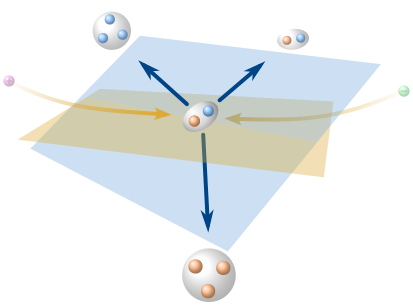
\includegraphics[width=0.8\textwidth]{images/aligning-baryons}
    \vskip 0cm plus 2fill
    \begin{otherlanguage}{german}
      \large
      {\scshape Dissertation}\par
      zur\par
      Erlangung des Grades eines\par
      Doktors der Naturwissenschaften\par
      an der Fakultät für Physik und Astronomie\par
      der Ruhr-Universität Bochum\par
      \vspace{4ex}
      von\par \vspace{0.2em}
      {\Large\bfseries Remco Emiel de Boer}\par \vspace{0.2em}
      aus Wageningen (Niederlande)\par
      \vspace{8ex}
      Bochum, $date$\par
    \end{otherlanguage}%
  }
  \vspace*{\fill}
\end{adjustwidth}
$endif$

\custompagebreak
\thispagestyle{empty}
\vspace*{\fill}

\begin{tabular*}{0.7\textwidth}{@{}l@{\extracolsep{\fill}}l@{}}
  1. Gutachter          & Prof.\ Dr.\ Miriam Fritsch     \\[1.5em]
  2. Gutachter          & Prof.\ Dr.\ Mikhail Mikhasenko \\[1.5em]
  Datum der Disputation & 1. Dezember 2025
\end{tabular*}
